%\jules{ Draw the reader in, by exposing the problem and its importance in the field today, the problem being optimizing queries whose output is semi-structured. Ideally, try to bring forth arguments why this will become a larger and larger problem in the future. }
There has been a rise in interest over the last few years in querying and producing semi-structured, hierarchical data. Document databases, which query and produce documents with nested structure (such as MongoDB, AsterixDB and CouchDB), are being increasingly utilized for use cases ranging from operational and analytical intelligence to web application development. As a testimony to this growth, the NoSQL database market is expected to increase to over four billion dollars by 2020 \cite{asay:2015}. ETL Data integration middlewares that are used to insert into those database also process queries with nested results. The queries that have to be answered by those systems are inherently non-relational, and require query optimization techniques adapted to hierarchical data.

% \jules{Specify the contribution. Review of query decorrelation literature, with a focus on query decorrelation on semi-structured data, Outline our improvements: query decorrelation without an ID, performance improvements and improvement upon analytical queries.}
This paper focuses one particular optimization, query decorrelation for semi-structured query processing. Query decorrelation has been studied extensively in the relational context \cite{kim-tods-82, dayal-vldb-87, muralikrishna1989optimization, ganski-sigmod-87} where the subquery occurs in the \texttt{WHERE} clause; while fewer works have focused on the \texttt{SELECT} clause, given its limited applicability in the context of SQL \cite{galindo-legaria:2001aa}. Previous solutions have however been provided in the context of XQuery \cite{may:2003aa}, where subqueries in the \texttt{return} clause are allowed. Nevertheless, the existing solutions have some performance limitations in the presence of 1) duplicates in the outer query and 2) joins in the subquery. Moreover, no prior published work has tackled the problem when those subqueries are analytical in nature (i.e. they contain grouping/aggregation, sorting and top-k operations). We address both problems in this paper by introducing a set of algebraic equivalences which improve on prior work.

% \jules{Introduce SQL++ briefly and show improvements clearly through an example.}
One first difficulty which arises when developing query optimization techniques for semi-structured data is the lack of standard query language across the semi-structured query processors. Ong. et al \cite{} showed that the various languages of SQL-on-Hadoop, NoSQL and NewSQL databases can be accurately modeled by a unifying, SQL backwards-compatible language called SQL++. SQL++ is most easily defined by removing restrictions from SQL semantics. Of particular interest is the ability to have any kind of SQL subquery in the \texttt{SELECT} clause, potentially creating nested results. We will be using SQL++ for examples throughout the paper. 

\begin{minipage}{\linewidth}
\lstinputlisting[language=SQL,label={list:running},caption={Analytical query and schema for a large web store},escapeinside={(*}{*)}]{code/running_example.sql}
\end{minipage}

On figure \ref{list:running} is shown a SQL++ nested query typical of an analytical intelligence use case over a large web store. The schema for the query is taken from the BigBench \cite{ghazal:2013aa} benchmark. For the first L promotions, an analyst wants to identify the top 3 promotions over the same item in terms of web sales revenue. Notice that the 1) the subquery is parameterized with the outer promotion table reference \texttt{@p1} and 2) the subquery will return a collection of tuples with two attributes each, one for the promotion name and one for the revenue, which would make it invalid in the SQL context. 

% Paragraph 1 : TAAT is known to suck in terms of performance, and this problem has been addressed for a long time. 
The execution that is closest to the query formulation is to compute the \texttt{top\_web\_sales} value using a separate subquery for each promotion tuple which satisfies the \texttt{WHERE} clause condition. This is commonly considered an poor strategy, as it involves \emph{tuple-at-a-time} processing of the subquery.  A much more efficient query execution strategy is made possible by decorrelating the subquery, allowing the entire set of subqueries to be processed at once, hence the name \emph{set-at-a-time} execution.

% \jules{Show existing work based on describing the DSAAT execution. Show how the partition by operations makes analytical queries possible. Show why performance sucks.}

On figure \ref{fig:DSAAT_example} is shown an algebraic representation of the denormalized set-at-a-time execution. This execution plan improves on top of the work of May et al. \cite{may:2003aa} by providing set-at-a-time semantics for SQL++ analytical clauses \texttt{GROUP BY}, \texttt{ORDER BY} and \texttt{LIMIT} within the subquery.

% Describe the DSAAT algebraic plan execution.
The outer query's \texttt{FROM} and \texttt{LIMIT} clauses are processed on the left hand side of the left outer join, using the \texttt{LAMBDA. On the right hand side of the left outer join, the \texttt{FROM} clause of the subquery is processed. The left outer join then processes the subquery \texttt{SELECT} clause. 



\begin{figure}[h]
\centering
\caption{Denormalized Set-At-A-Time execution \label{fig:DSAAT_example}}
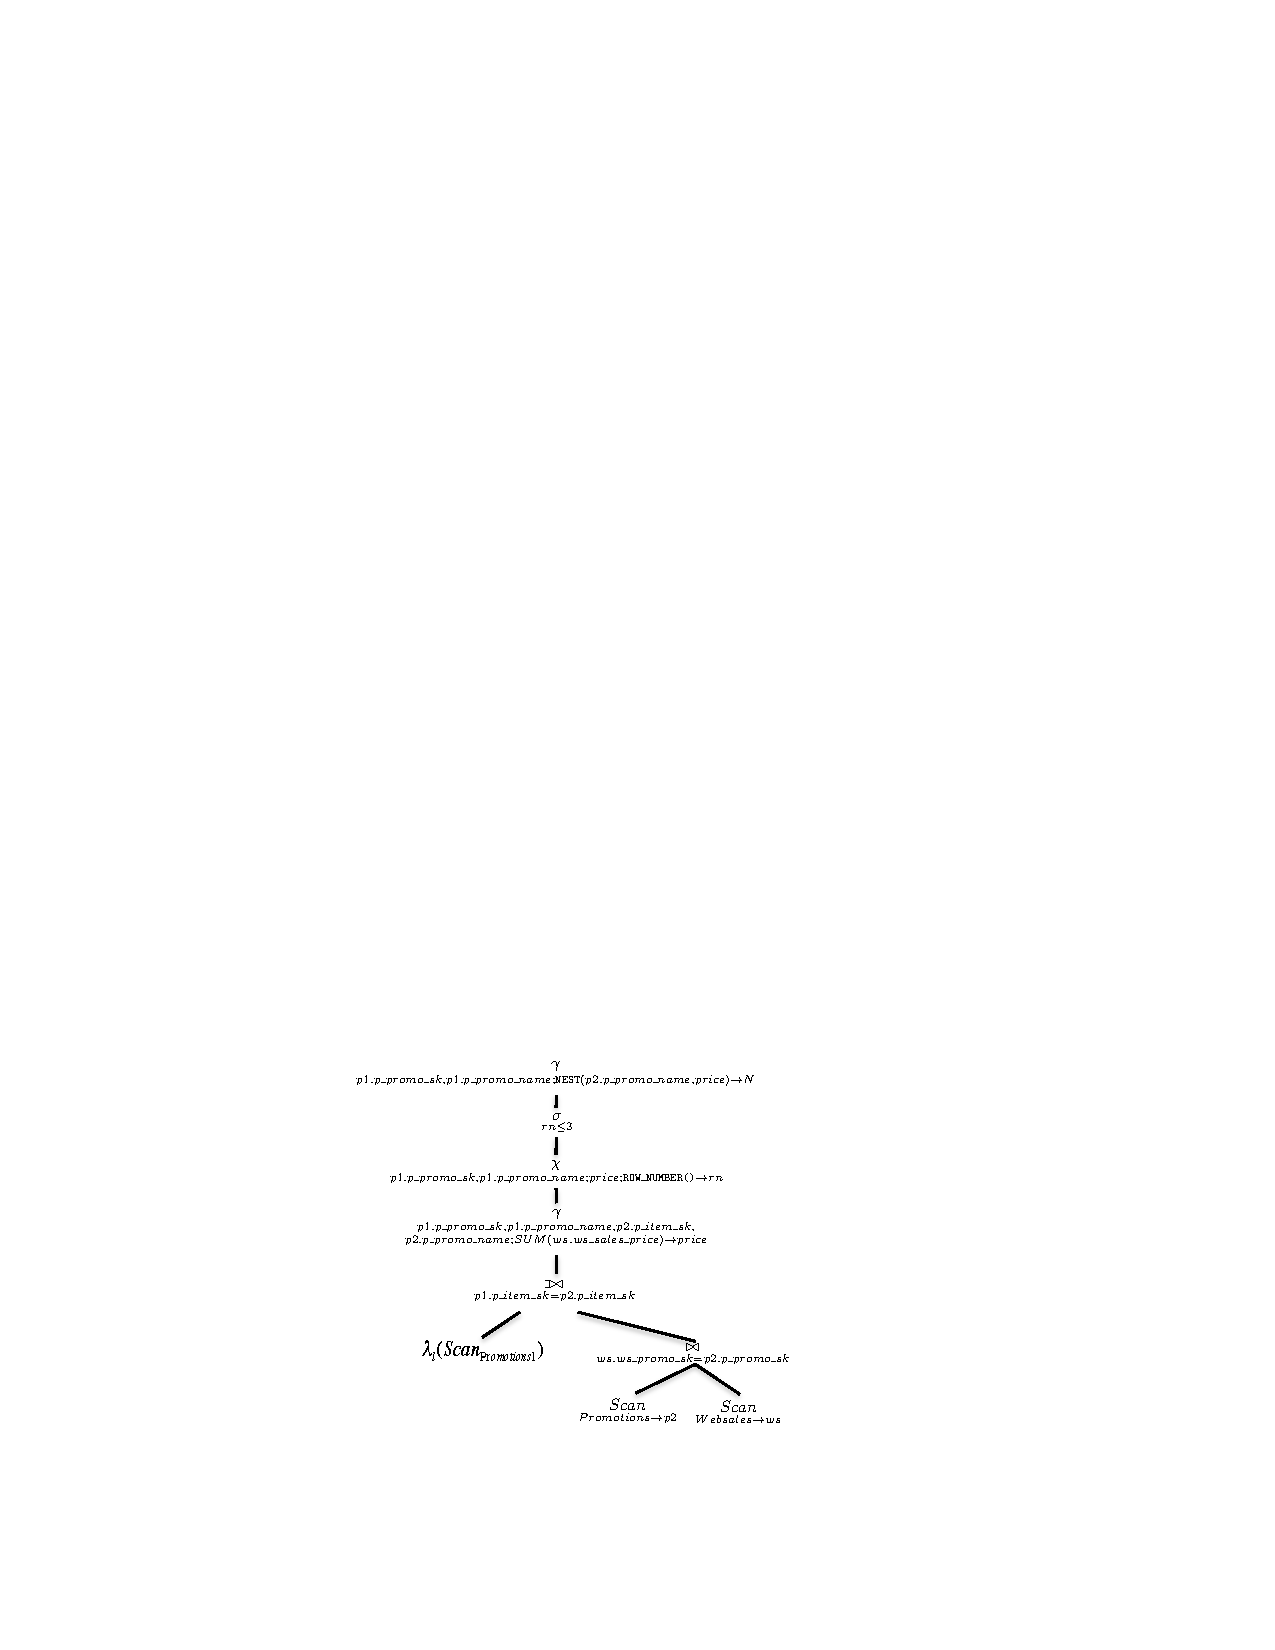
\includegraphics[width=1.05 \linewidth]{images/DSAAT_running-example.pdf}
\end{figure}

Notice that in the running example, there is a functional dependency from the correlated attribute \texttt{p\_item\_sk} to the attributes \texttt{p\_promo\_name} and \texttt{price} of \texttt{top\_web\_sales}. The $\leftouterjoin$ denormalizes intermediate results by joining on \texttt{p\_item\_sk}, thus introducing more non-correlated attributes from its left hand side. This creates two types of performance penalties: 1) horizontal redundancy 


\jules{Show NSAAT and how it improves upon DSAAT by outlying performance improvements.}

We introduce a normalized-set rewriting on figure \ref{NSAAT_example}. It introduces the $Scan$ and $\delta$ operators (which is reminiscent of the classical semi-join technique in distributed query processing), and deferring the $\leftouterjoin$ until all analytical operators are processed.

\begin{figure}[h]
\centering
\caption{Normalized Set-At-A-Time execution \label{fig:NSAAT_example}}
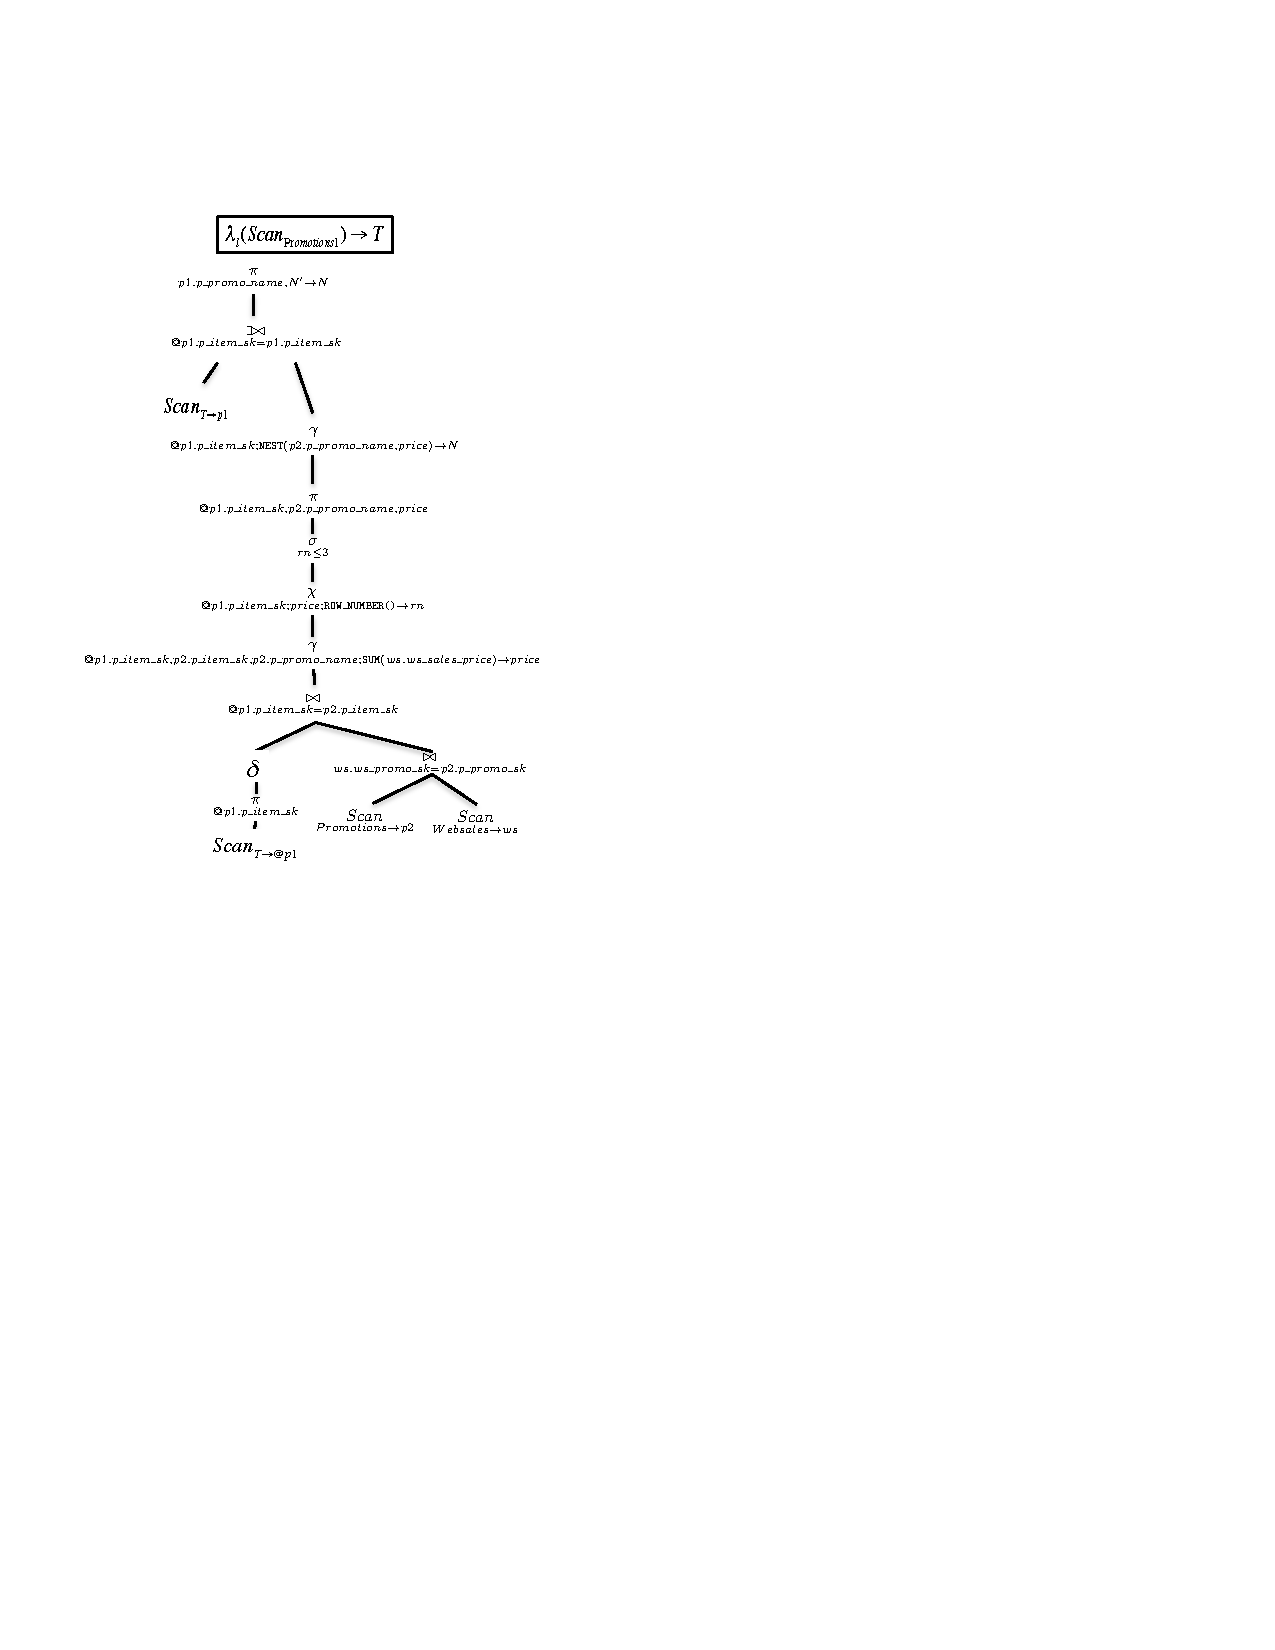
\includegraphics[width=1.05 \linewidth]{images/NSAAT_running-example.pdf}
\end{figure}

\jules{Outline and contributions}


\jules{The key requirement for DSAAT is only necessary because the $\gamma_{\texttt{NEXT}()}$ is happening above the left outer join. If the $\gamma_{\texttt{NEXT}()}$ is placed below the left outer join, the key requirement is no longer necessary but the performance may degrade because aggregation happens before the left outer join, which may be filtering}

\jules{@Yannis: One question that could arise is whether it is necessary that the input data to the query be relational, since it is in our running example. In particular, what happens if the correlation attributes are nested or missing for some or all tuples.}

\jules{The May paper \cite{may:2003aa}  uses the $\chi$ symbol for their apply plan operator and the $\alpha$ symbol to mean the head of a list. I hope our use of the same symbols for different operators won't confuse our readers early on.}

\jules{Unfortunately, there is no equivalent to the  \texttt{LIMIT} keyword in the SQL standard, each DBMS having it's own syntax. My introduction assumes the semantics of \texttt{LIMIT} are obvious.}